% https://tex.stackexchange.com/q/639726/86
\documentclass[tikz,border=5pt]{standalone}
\usetikzlibrary{spath3}
\begin{document}

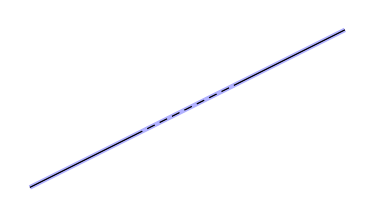
\begin{tikzpicture}

\draw[spath/save=path,ultra thick,blue!30] (0,0) -- (4,2);
\draw[spath/split at keep start={path}{1/3},spath/use=path];
\draw[spath/split at keep end={path}{2/3},spath/use=path];
\draw[spath/split at keep middle={path}{1/3}{2/3},spath/use=path,densely dashed];
\end{tikzpicture}

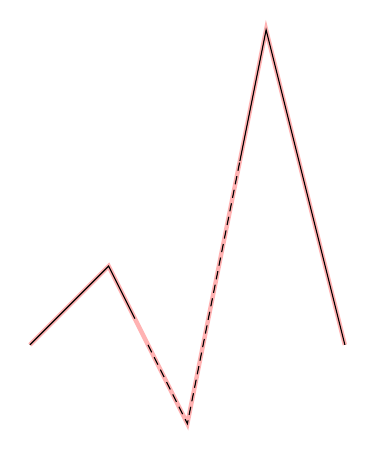
\begin{tikzpicture}

\draw[spath/save=path,ultra thick, red!30] (0,0) -- (1,1) -- (2,-1) -- (3,4) -- (4,0);
\draw[spath/split at keep start={path}{1/3},spath/use=path];
\draw[spath/split at keep end={path}{2/3},spath/use=path];
\draw[spath/split at keep middle={path}{1/3}{2/3},spath/use=path,densely dashed];
\end{tikzpicture}
\end{document}